
\noindent \textcolor{COLOR1}{Questão 05)} Realize o seguinte experimento para compressão de imagens
usando decomposição SVD. No Python, digite as seguintes linhas de comando:
\\

\begin{lstlisting}
# Importar a biblioteca de imagens
import matplotlib.pyplot as plt
import matplotlib.image as mpimg 
import numpy as np 

img = mpimg.imread('pirata.png') # Lendo o arquivo da imagem 
original
plt.figure() # Criando uma figura
imgplot = plt.imshow(img, cmap='gray') # Plotando a imagem 
original
plt.title('Original') # Titulo da imagem
plt.axis('off') # Desabilitando os eixos
U, S, V = np.linalg.svd(img) # Realizando a decomposicao SVD
postos = [10, 30, 50, 100, 200] # Lista de postos para a 
compressao

for posto in postos: # Para cada posto
    aproxSigmas = S[0:posto] # Aproximando os valores de S
    aproxS = np.diag(aproxSigmas, 0) # Criando a matriz diagonal
    aproxU = U[:, 0:posto] # Aproximando os valores de U
    aproxV = V[0:posto] # Aproximando os valores de V
    aproxImg = aproxU @ aproxS @ aproxV # Criando a imagem 
    aproximada
    plt.figure() # Criando uma figura
    aproxImgplot = plt.imshow(aproxImg, cmap='gray') # Plotando
     a imagem aproximada
    plt.title('Aproximacao de posto ' + str(posto)) # Titulo da
     imagem com posto
    plt.axis('off') # Desabilitando os eixos
\end{lstlisting}

\begin{figure}[htbp]
    \centering
    \subfloat{{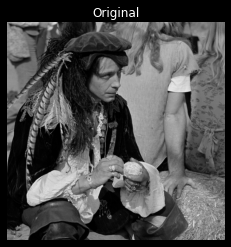
\includegraphics[scale=.8]{/metodos/original.png} }}%
    \quad
    \subfloat{{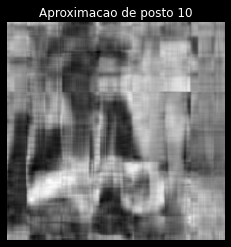
\includegraphics[scale=.8]{/metodos/posto10.png} }}%
    \quad
    \subfloat{{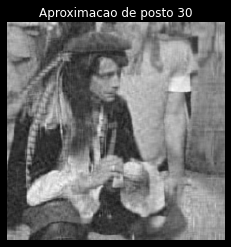
\includegraphics[scale=.8]{/metodos/posto30.png} }}%
    \quad
    \subfloat{{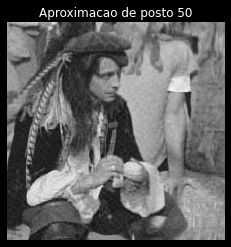
\includegraphics[scale=.8]{/metodos/posto50.png} }}%
    \quad
    \subfloat{{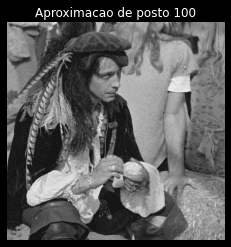
\includegraphics[scale=.8]{/metodos/posto100.png} }}%
    \quad
    \subfloat{{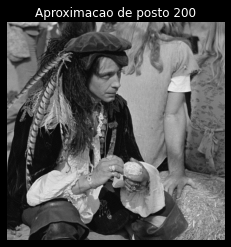
\includegraphics[scale=.8]{/metodos/posto200.png} }}%
\end{figure}


\begin{itemize}
    \item Você consegue explicar o que cada linha acima está mandando o Python fazer?
    \item Execute as linhas acima e observe os resultados.
    \item Para cada posto considerado determine a quantidade de números que devem ser armazenados na aproximação da imagem e compare com a quantidade de números necessários para armazenar a imagem original. Analise as imagens obtidas para postos diferentes.
\end{itemize}

Para a análise de imagens, utilza-se do código em python a seguir:\\

\begin{lstlisting}
# Importar a biblioteca de imagens
import matplotlib.image as mpimg
import numpy as np
    
img = mpimg.imread('pirata.png')
U, S, V = np.linalg.svd(img) 
postos = [10, 30, 50, 100, 200]
    
print("Imagem original tem dimensao: {}x{}\n".format(
        img.shape[0], img.shape[1]))
print("Imagem original tem armazenamento: {}".format(
        img.shape[0]*img.shape[1]))
for posto in postos:
    print("Imagem do posto {} tem armazenamento: {}".format(
        posto, posto * (img.shape[0]+img.shape[1]+1)))

#Imagem original tem dimensao: 512x51

#Imagem original tem armazenamento: 262144
#Imagem do posto 10 tem armazenamento: 10250
#Imagem do posto 30 tem armazenamento: 30750
#Imagem do posto 50 tem armazenamento: 51250
#Imagem do posto 100 tem armazenamento: 102500
#Imagem do posto 200 tem armazenamento: 205000
\end{lstlisting}